\begin{figure*}[t!]
\begin{center}\footnotesize
	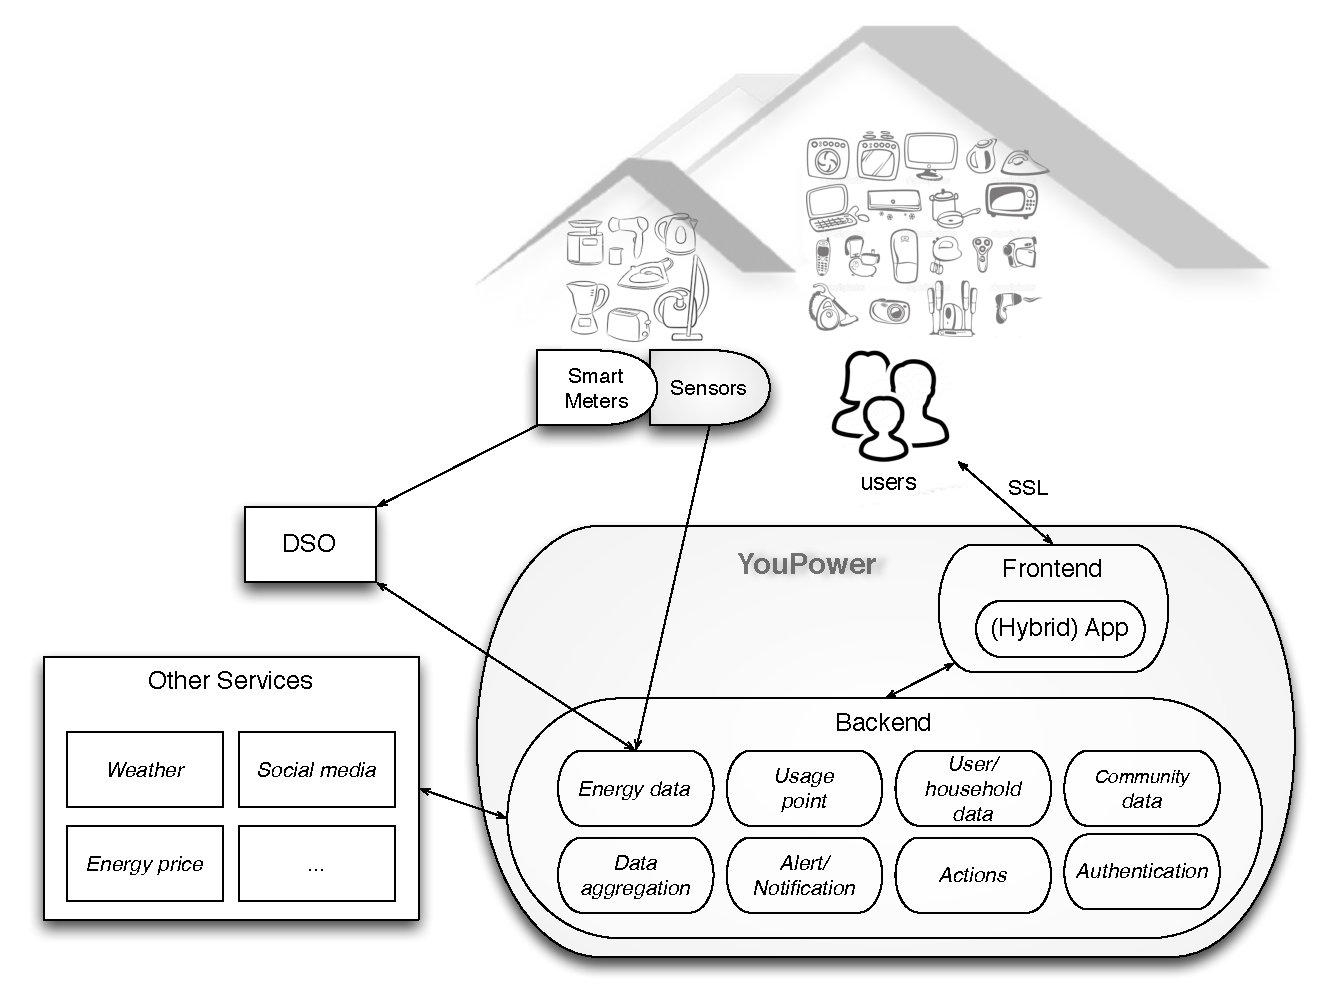
\includegraphics[width=.7\textwidth]{img/civis_platform_overview.pdf}\\
	DSO (Distribution System Operators),  SSL (Secure Sockets Layer)
	\caption{YouPower system overview}\label{fig:platform}
\end{center}
\end{figure*}

\section{\uppercase{State of the Art}}

\noindent Prior to designing YouPower, we review the existing studies with social smart grid platforms and summarize the lessons learned from those studies. Combining such lessons with findings from the literature on pro-environmental behavior change we compile a set of design guidelines with successful strategies and potential barriers for social energy platforms. For instance, a repeatedly reported issue with such platforms is a lack of long term user engagement \cite{edward2015review}. We adopt iterative, open and lean co-design process \cite{folstad2008living,klein2013ux} that is suggested as a promising approach to avoid this issue \cite{schwartz2014people}.

\paragraph{Existing social energy platforms.} Weiss et al.~\cite{weiss2012powerpedia} developed a smartphone community platform, PowerPedia. The platform works in connection with smart meters and enables users to identify, upload and compare their appliance-level consumption data. The test users rated favorably social comparison features and appliance level statistics. Community Monitor \cite{dillahunt2014understanding} featured leaderboard, message board and shared actions ("ways to save"). The findings from the 4-10 months trial revealed the importance of environmental and social context for social energy apps. For instance, the existence of common spaces for community members to interact and knowledge of other users supported the app use. Petkov et al.~\cite{petkov2011motivating} investigated comparative consumption feedback. Their findings confirm the importance of comparison to the similar users. However, if the competition features are included, then the users preferred to compete with the people whom they actually know, such as friends.

\paragraph{Design ideas and guidelines.} The literature review suggests that the most successful behavior change interventions combine several different strategies \cite{gardner1996environmental,ockwell2009reorienting}. However, a special care must be taken to avoid mixed messages \cite{knowles2014patterns}, especially when combining intrinsic and extrinsic motivations \cite{delmas2013information}. Additionally, the literature agrees that there is no a silver-bullet type of a solution and that we need interventions carefully \textit{attending to the context} \cite{hargreaves2013keeping,dillahunt2014understanding}.

Most of the solutions involve some type of \textit{consumption feedback}, such as historical or real-time (individual or group). Introduction of descriptive or injunctive \textit{social norms} through comparative feedback has proven effective \cite{allcott2011social,cialdini2001harnessing,petkov2011motivating}. Additionally, Strengers \cite{strengers2011designing} suggests combining feedback with \textit{practical recommendations (tips)} that lead to new practices which challenge taken-for-granted notions of normality. Several studies \cite{abrahamse2005review,delmas2013information} report tailored energy advice to a specific household and personalized information to be the most effective strategy. Another effective strategy that applies social dimension is \textit{public commitment} \cite{abrahamse2005review}, a procedure in which people are binding to a certain behavior. One suggestion to increase the effectiveness is to \textit{target organisations, companies and policy makers} \cite{hasselqvist2015supporting,brynjarsdottir2012sustainably} in addition to individuals.
Next, we describe how each of the strategies above is incorporated into the design of YouPower (for the full set of our design guidelines, refer to CIVIS D3.2.).

X Considering the recommendation to attend to the intervention context and the analytical frames above, we chose a set of platform features and translated those into three self-contained and composable parts so that each part will support different CIVIS use-cases and the specific socio-economic contexts in Stockholm and Trentino. The three parts included in the CIVIS (front-end) application (hereinafter abbreviated as CIVIS app) are: 
%\begin{enumerate}
%\item \nameref{sect:tips}
%\item \nameref{sect:brf}
%\item \nameref{sect:load_shifting}
%\end{enumerate}

The Energy Data Visualization part of YouPower incorporates both individual and group (household and community) feedback. The community feedback informs about a collective effort and might enhance the feeling of group efficacy \cite{bandura1997self}. In YouPower, the special attention is given to the household context, since bringing \textit{family values into discussion} and establishing \textit{shared commitments and responsibilities} is reported to be effective \cite{huizenga2015shedding}. Additionally, the BRF part of the app applies social norms through comparison between the housing cooperatives. The BRF part also involves energy managers, who have the power to significantly influence the practices related to energy use. The Action Suggestions part not only teaches users about sustainable energy practices, but also applies public commitment strategy through making visible the actions that the user takes.

With peer review results and users' feedback on the design, adaptations and changes are made to suit user needs and to achieve the CIVIS research goal. 
In general, the application aims to enhance users' energy know-how through action suggestions that are implementable in everyday life, engage users in energy communities with understandable and actionable information and feedback, and facilitate community interaction and self-teaching by means of group discussions.

Given the time and resource constraints, the app can not be developed all-in-one cross-platform (for phones, tablets and computers). We chose to design the front-end as a mobile app. This means that the app design has layouts and user interactions that suit (small) phone screens. %The consideration is multi-fold. 
Western Europe has a large mobile phone internet user base\footnote{
Between 2013 and 2017, the penetration rate of mobile phone internet users among mobile phone users will rise from 49.0\% to 77.8\%. See more at: \url{ http://www.emarketer.com/Article/Nearly-Half-of-Western-Europeans-Will-Use-Mobile-Web-This-Year/1010510\#sthash.AaVfsqIU.dpuf}}. Many surveys show that mobile apps have advantages such as creating deeper user engagement, easy sharing, among others\footnote{\url{https://infomedia.com/blog/the-advantages-of-mobile-apps/}, \url{https://econsultancy.com/blog/62326-85-of-consumers-favour-apps-over-mobile-websites/}}. This makes mobile app a good choice given the goal of the CIVIS platform. Once developed, mobile apps can also be more easily transformed to web browser versions, while the reverse is more difficult. The back-end of the CIVIS platform will remain mostly the same independent of the front-end alternatives. 